\begin{figure}[!htb] 
\centering 
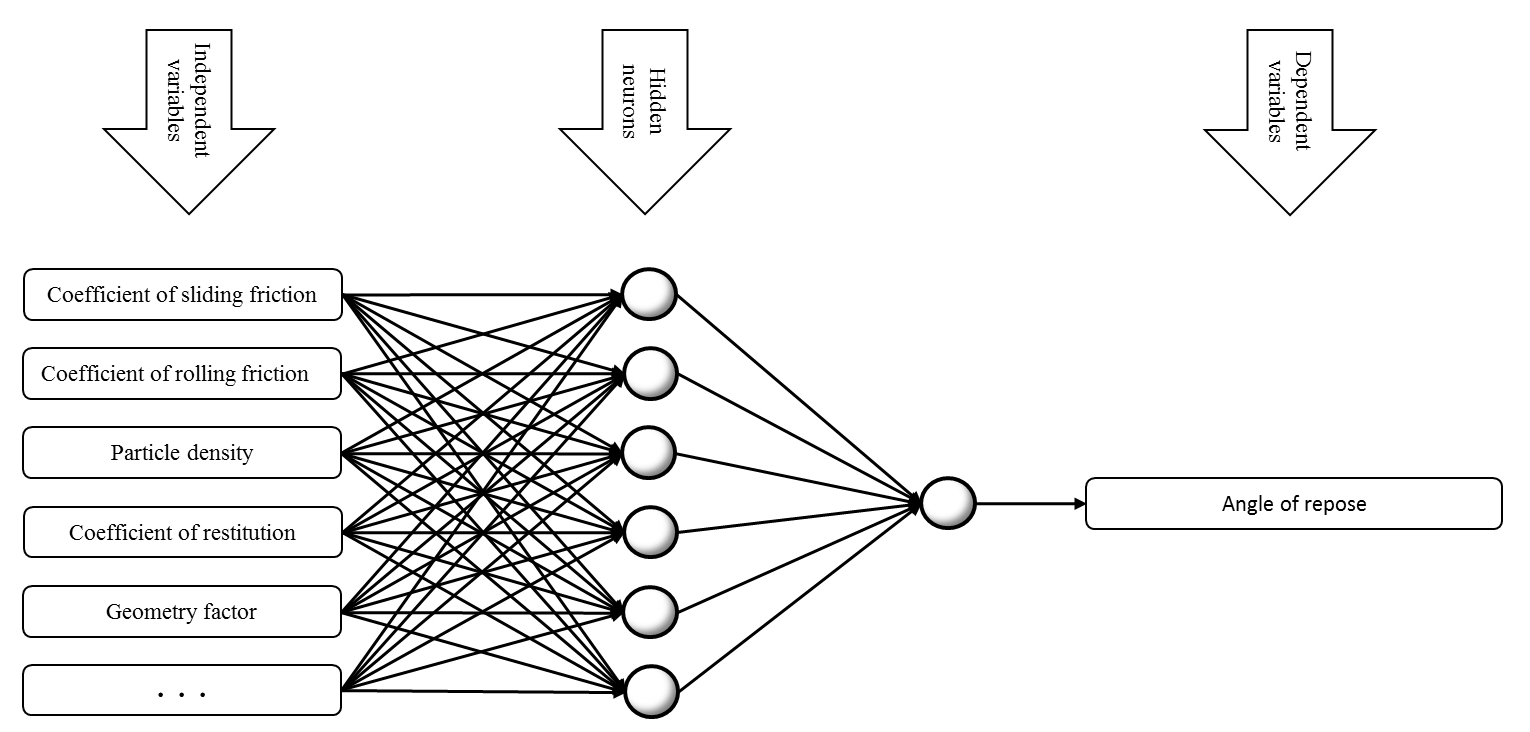
\includegraphics[width=.96\textwidth]{images/original/18nnscheme} 
\caption[NN Scheme]{Neural Network ($NN$) Scheme. This is the schematic of how
the Multi Layer Perceptron $NN$ ($MLPNN$) derives one bulk behaviour
dependent variable from the mutually independent simulation variables.}
\label{fig:18nnscheme} 
\end{figure}


% \begin{figure}[htp]
%     \centering
%     
\includegraphics[width=.2\textwidth]{images/vitae/lbenvenuti}
%     \caption{OpenMP, MPI, MPI/OpenMP Hybrid runs of Box in a box testcase on 32
%     cores. The OpenMP-only run suffers from limited memory bandwidth in
%     memory-bound algorithms inside of the Modify section of the code. MPI-only has
%     low averaged runtimes for each section, but a very large Other timing, which
%     hints for a large amount of load-imbalance. Hybrid timings are a bit worse
%     on average, but because of better balancing, processes have lower wait times
%     inside of Other timing.}
% 	\label{fig:boxInBoxComparison}
